\section{Theorie}
\label{sec:Theorie}
In diesem Versuch sollen mittels optischen Pumpens die Kernspins $I$ der Isotope $^{85}$Rb und $^{87}$Rb bestimmt werden. Rb ist das Element Rubidium, welches ein Alkalimetall ist.

\subsection{Landé-Faktoren}

Ein Teilchen, das sich wie ein Elektron in einem Atom bewegt, besitzt einen Drehimpuls $\vec L$ bei der Bewegung um den Kern.
Der Spin $\vec S$, eine Größe, die aus der relativistischen Quantenmechanik resultiert, charakterisiert das Teilchen neben seiner Masse und Ladung. 

Beide Größen, Drehimpuls $\vec L$ und Spin $\vec S$, besitzen ein magnetisches Moment, das sich als 
\begin{align*}
    \mu_\text{L} &= \mu_\text{B} \, g_\text{L} \, \sqrt{L(L+1)} \\ 
    \mu_\text{S} &= \mu_\text{B} \, g_\text{S} \, \sqrt{S(S+1)}
\end{align*}
darstellen lässt mit dem Bohrschen Magneton $\mu_\text{B}$ und den Landé-Faktoren $g_\text{L,S}$ \cite{pfeiler}. 

Da die Bewegung des Elektrons ein magnetisches Feld erzeugt und der Spin, der eine magnetische Größe ist, insofern mit diesem Magnetfeld interagiert, koppeln der Spin und der Drehimpuls miteinander. 
Die resultierende Größe ist der Gesamtdrehimpuls $\vec J = \vec L + \vec S$ \cite{pfeiler}.

Auch hier ergibt sich ein magnetisches Moment $\vec \mu_\text{J}$, das um die Richtung des Gesamtdrehimpulses präzediert, wobei der senkrechte Anteil im Mittel herausfällt und nur der parallele Anteil relevant ist. 
Für $\vec \mu_\text{J}$ ergibt sich 
\begin{equation*}
    \mu_\text{J} = \mu_\text{B} \, g_\text{J} \, \sqrt{J(J+1)}
\end{equation*}
und für $g_\text{J}$ gilt 
\begin{equation}
    g_\text{J} = 1 + \frac{J(J+1) + S(S+1) - L(L+1)}{2J(J+1)}
    \label{eq:gj}
\end{equation}
bei einer vektoriellen Betrachtung der magnetischen Momente und der dazugehörigen Größen $\vec J$, $\vec L$ und $\vec S$ \cite{caltech}.

\subsection{Energieaufspaltung}
Eine schematische Darstellung der Energieaufspaltung bei den hier betrachteten Rubidium-Isotopen ist in Abb. \ref{fig:Aufspaltung} zu sehen.

Durch die Spin-Bahn-Kopplung werden die Energieniveaus zum ersten mal gespalten, je nachdem in welche Richtung der Drehimpuls und der Spin gerichtet sind (parallel, orthogonal oder antiparallel).
Diese Aufspaltung nennt sich Feinstruktur. \cite{pfeiler}

Die Energieverschiebung ergibt sich dann mit 
\begin{equation*}
    \Delta E = g_\text{J} \, \mu_\text{B} \, B \, m_\text{J},
\end{equation*}
wobei $m_\text{J}$ die Magnetquantenzahl ist. \cite{pfeiler}

Die Hyperfeinstruktur spaltet die Energieniveaus ein weiteres mal. 
Dabei kommt der Kernspin $I$ des Atoms in Spiel, wenn dieser von Null verschieden ist.
Die Kopplung $\vec F = \vec J + \vec I$ nimmt Werte von $| I - J|$ bis $I+J$ an. 
Mit einem Magnetfeld können diese Energieniveaus weiter gespalten werden, da das Magnetfeld auf die Hülle des Atoms wirkt, sodass sich $2F+1$ Unterniveaus ergeben. 
Dabei ist die Energieverschiebung 
\begin{equation*}
    \Delta E_\text{Zeeman} = g_\text{F} \, \mu_\text{B} \, B \, \Delta m_\text{J}.
\end{equation*}
\cite{caltech}

Der neue Landé-Faktor $g_\text{F}$ (\cite{caltech}) ist 
\begin{equation}
    g_\text{F} = g_\text{J} \frac{F(F+1) + J(J+1) - I(I+1)}{2F(F+1)}.
    \label{eq:I}
\end{equation}

\begin{figure}
    \centering
    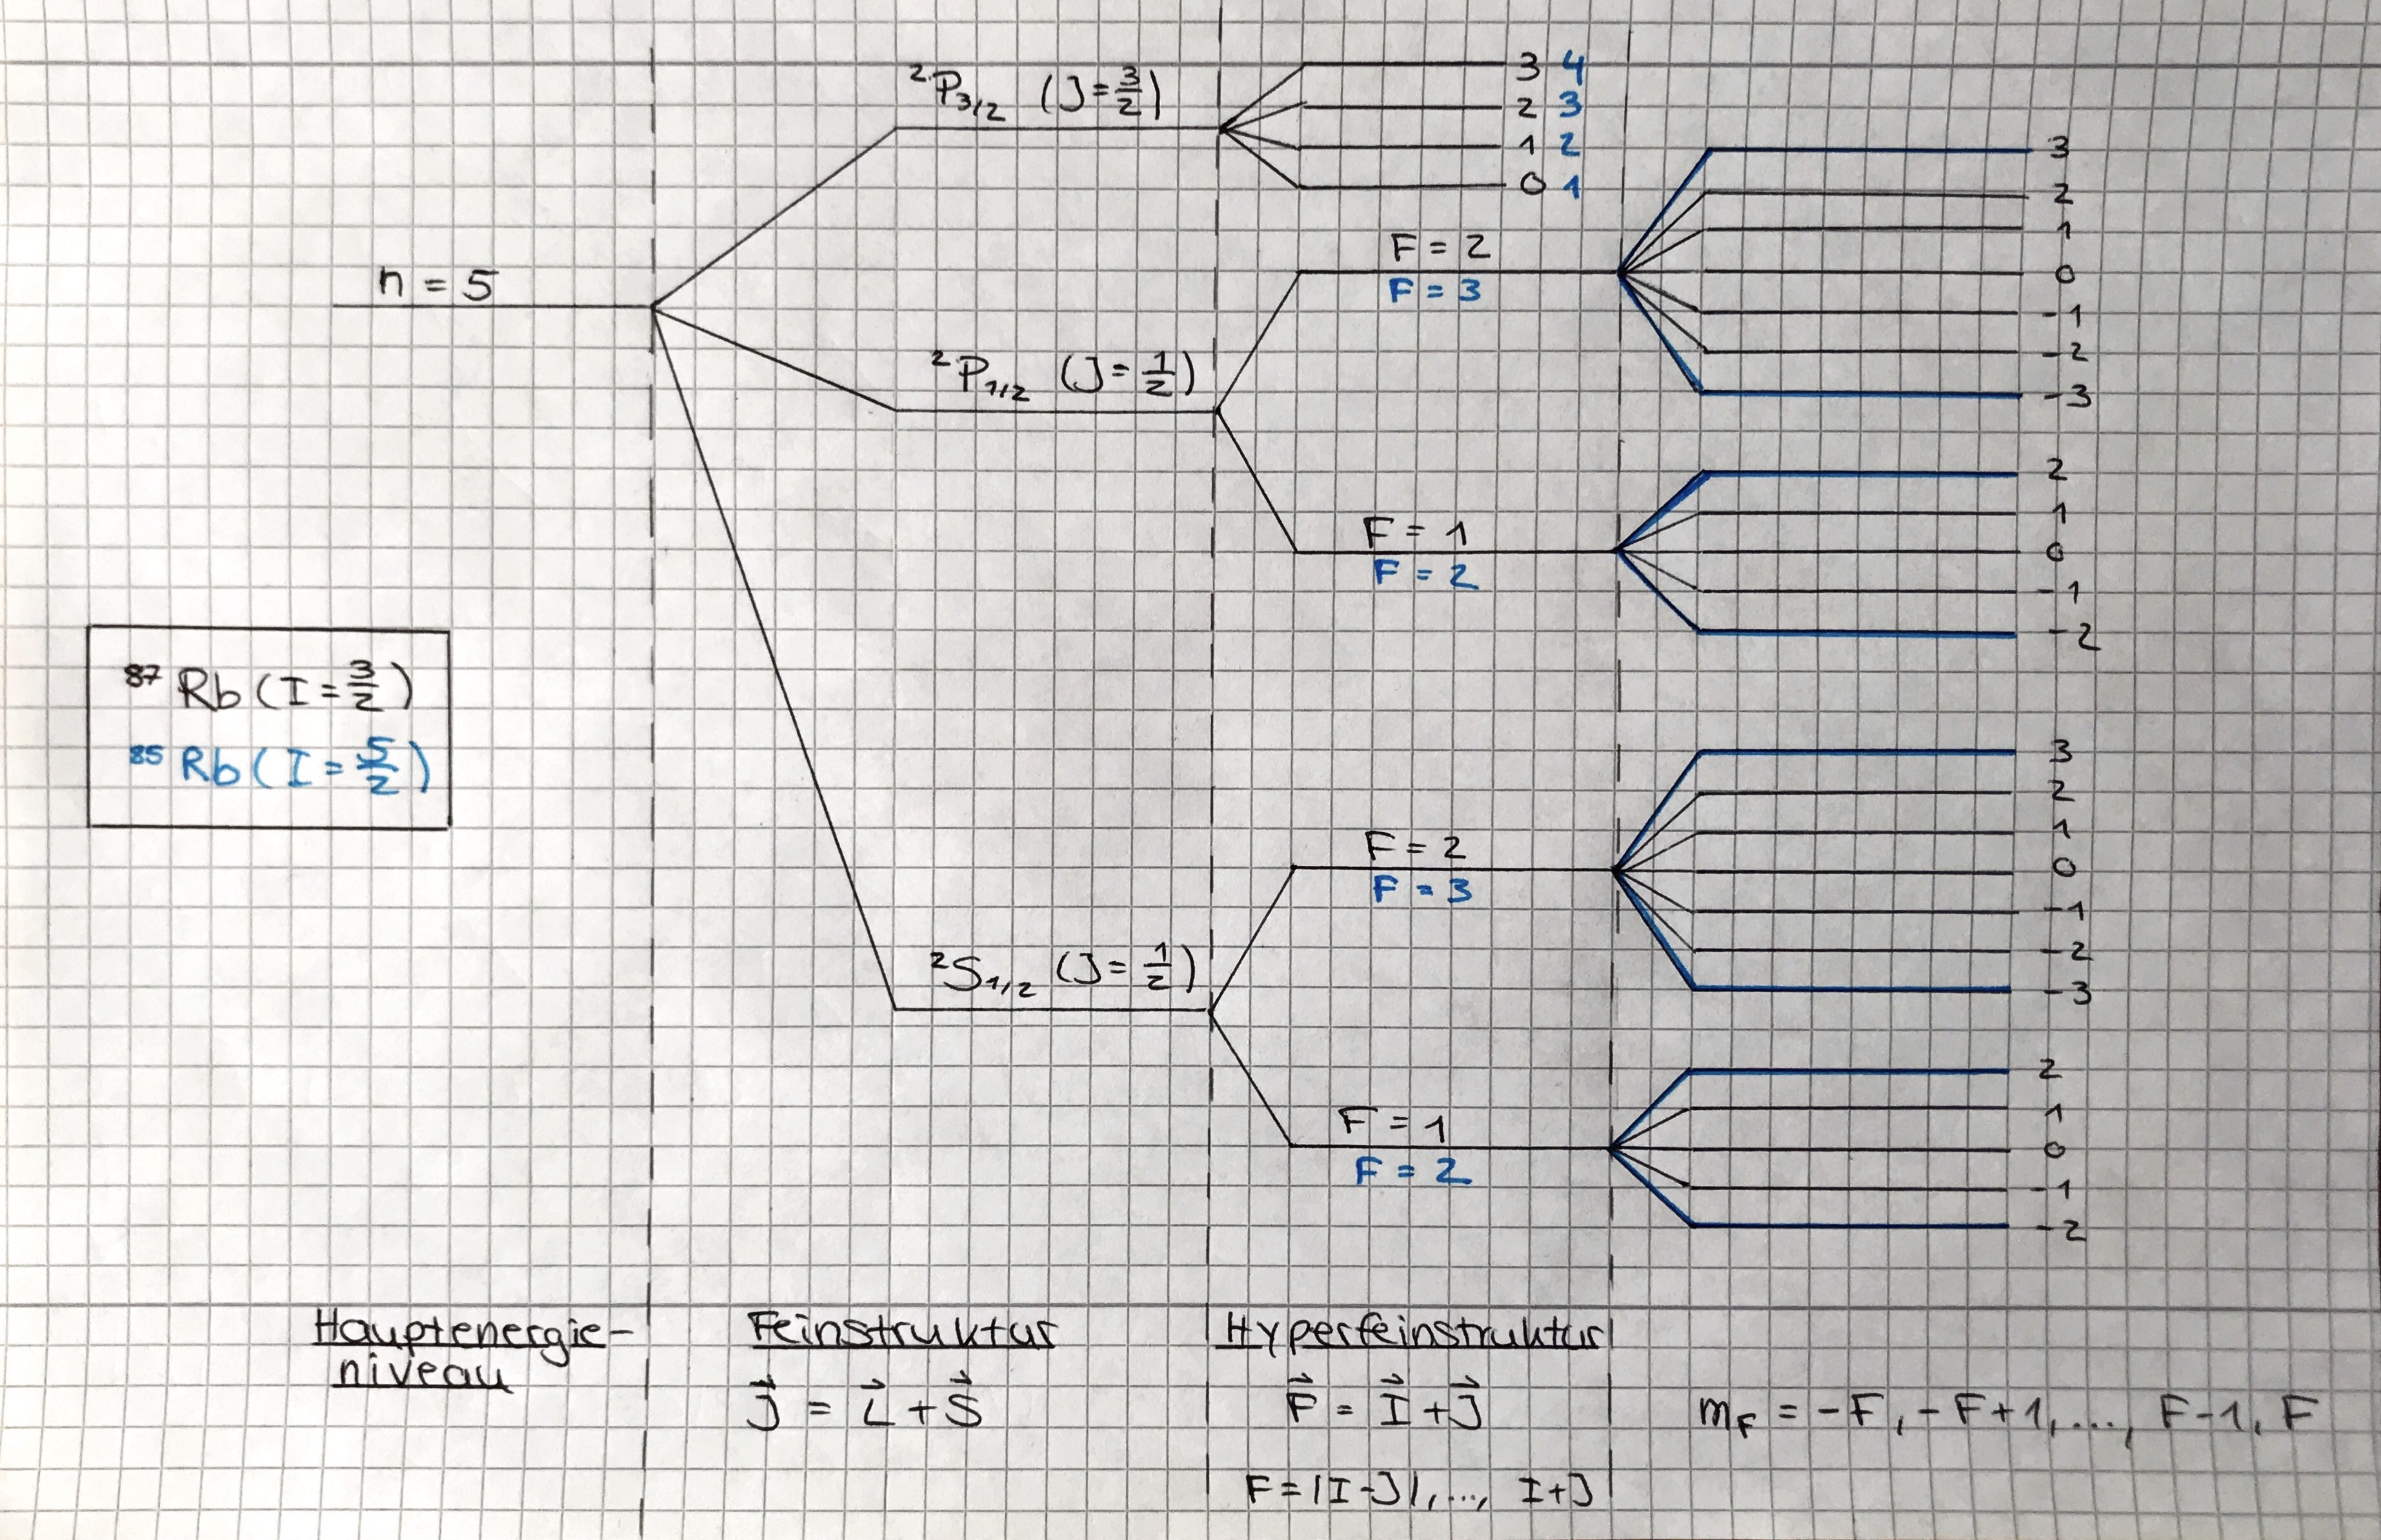
\includegraphics[width=15cm]{fotos/Aufspaltung.JPG}
    \caption{In dieser Skizze ist die Energieaufspaltung von $^{87}$Rb bzw. $^{85}$Rb (blau) zu sehen.}
    \label{fig:Aufspaltung}
\end{figure}

\subsection{Optisches Pumpen}

Um die einzelnen Energieniveaus zu messen, wird die Methode des optischen Pumpens genutzt. Dabei werden die Elektronen aus einem der zwei niedrigen Niveaus in ein höheres Niveau angeregt. 
Anschließend wird dieses Niveau wieder geleert mittels (spontaner und induzierter) Emission und in nur in eines der beiden niedrigen Niveaus gefüllt. \cite{caltech}

Es gibt $\sigma^+$- (rechtszirkular polarisiertes Licht), $\sigma^-$- (linkszirkular polarisiertes Licht) und $\pi$-Übergänge (linear polarisiertes Licht), die jeweils bestimmte Magnetquantenzahlen $\Delta m_\text{J}$ mit sich bringen (+1, -1, 0). \cite{pfeiler}


Dadurch erhöht sich die Transparenz. 

Für bestimmte Resonanzen des Magnetfelds, also genau dann, wenn 
\begin{equation}
    \Delta E_\text{Zeeman} = h \nu = g_\text{F} \, \mu_\text{B} \, B \, \Delta m_\text{J}
    \label{eq:Zeeman}
\end{equation}
ist, sinkt die Transparenz wieder. In diesem Versuch wird rechtszirkular polarisiertes Licht verwendet, also ist $\Delta m_\text{J} = \num{1}$.

Induzierte Emission ist ein Prozess, bei dem ein Photon eingestrahlt wird, welches genau die Energie der Differenz zwischen den beiden Niveaus besitzt. Dadurch treten dann zwei Photonen aus, die sich in Energie, Ausbreitungsrichtung und Polarisation nicht unterscheiden. \cite{pfeiler}
Die induzierte Emission ist hier der dominante Prozess aufgrund der niedrigen Frequenz der Zeeman-Aufspaltung.









